%\documentclass[professionalfonts]{beamer}
\documentclass[professionalfonts,handout]{beamer}
\usepackage[familydefault,light]{Chivo} 
\usepackage[T1]{fontenc}
\usenavigationsymbolstemplate{}
\usepackage[]{hyperref}
\usepackage{tikz,pgf,pgfarrows,pgfnodes,pgfbaseimage}
\graphicspath{{./Pics/}}
\usetikzlibrary{shapes}
\usepackage{setspace}
\newcommand{\evi}[1]{{\colorbox{yellow!50}{{#1}}}}
\newcommand{\exe}[1]{{\color{black!50}{{#1}}}}
\newcommand{\kw}[1]{{\colorbox{black!30}{\color{white}{#1}}}}
\tikzstyle{nd}=[circle,draw=black,thick,minimum size=.8cm,inner sep=1pt]
\setbeamercovered{transparent}
\usetheme{Singapore}
\tikzstyle{nodo}=[ellipse,draw=black!60,fill=black!10,line width=.7pt,minimum width=.7cm,minimum height=.4cm]
\usecolortheme[named=gray]{structure}
\setbeamercolor{block title}{bg=black!20,fg=black}
\setbeamercolor{block body}{bg=black!10,fg=black}

\title{Algoritmi Numerici (Parte I)}
\subtitle{[Lezione 3] Numeri razionali}
\author{Alessandro Antonucci\\{\tt alessandro.antonucci@supsi.ch}}
\date{\tiny\url{https://colab.research.google.com/drive/1Vz6HUgSJLjvMZCDgFlO8nrMYXECa310t}}
%%%%%%%%%%%%%%%%%%%%%%%%%%%%
\begin{document}
\maketitle
\frame{\frametitle{I Numeri Razionali e la Divisione}
\setstretch{1.4}
\begin{itemize}
\item Moltiplicazione \`e addizione iterata (col segno per interi)
\pause
\item \evi{Divisione} operazione inversa alla moltiplicazione
\pause
\item L'insieme degli interi non \`e chiuso rispetto alla divisione
$a,b\in\mathbb{Z}$ $\Rightarrow$ $\mathrm{DIVISIONE}(a,b) \in \mathbb{Z}$ solo se $|a|$ multiplo di $|b|$
\pause
\item Soluzione? Allargare l'insieme definendo $a/b$
\pause
\item L'insieme allargato $\mathbb{Q}$ si chiama dei numeri \evi{razionali}
\item I razionali si esprimono com rapporti di numeri interi (primi fra loro, $a/b$ e $(ka)/(kb)$ sono lo stesso numero)
\end{itemize}}



\frame{\frametitle{Quanti sono i numeri razionali?}
%\begin{columns}
%\begin{column}[T]{0.8\textwidth}
\begin{itemize}
\pause
\item Infiniti, ma in corrispondenza uno a uno con i naturali 
\pause
\item Ogni intero \`e razionale ($\mathbb{Z}\subseteq \mathbb{R}$) \exe{Es. 135 = 135/1}
\pause
\item Elementi $\mathbb{Q}$ su matrice con infinite righe e colonne
\vskip 2mm
$a/b \in \mathbb{Q}$ con $b>0$ su elemento di riga $a$ e colonna $b$
\vskip 2mm
\begin{tabular}{ccccccccc}
$\ldots$ & $\ldots$ & $\ldots$ & $\ldots$ & $\ldots$ & $\ldots$ & $\ldots$ & $\ldots$ \\
$\ldots$ & -3/3&  -2/3&  -1/3&   0/3&   1/3&   2/3&   3/3 & $\ldots$\\
$\ldots$ & -3/2&  -2/2&  -1/2&   0/2&   1/2&   2/2&   3/2 & $\ldots$\\
$\ldots$ & -3/1&  -2/1&  -1/1&   0/1&   1/1&   2/1&   3/1 & $\ldots$
\end{tabular}
\end{itemize}
\begin{center}
\pause
Algoritmo di ricopertura (a spirale) 
\vskip 1mm
produce corrispondenza con i naturali
\end{center}
}

\frame{\frametitle{Rappresentazione razionali in base 10}
\begin{center}
Se $a/b$ (non necessariamente ai minimi termini) tale che $b=10^k$
\vskip 1mm
il numero ha una rappresentazione decimale (finita)
\pause
\vskip 2mm
Es. $134.75 = \frac{13475}{100}$
\end{center}
\pause

Somma potenze positive (sx del punto) e negative (dx)
$134.75 = 134 + .75$
\\
$134= 1 \cdot 10^2 + 3 \cdot 10^1 + 4 \cdot 10^0$ \\$0.75 = 7 \cdot 10^{-1} + 5 \cdot 10^{-2}$
\pause
\begin{block}{Due Osservazioni}
\begin{enumerate}
\pause
\item La stessa cosa si pu\`o fare con basi diverse da 10
\pause
\item I numeri si possono leggere con l'algoritmo di Horner\\
(adattato al caso di potenze negative)
\end{enumerate}
\end{block}
}

\frame{\frametitle{Horner per i numeri ``frazionari''}
\begin{center}
Chiamiamo (solo in questo corso) frazionari\\ i numeri razionali positivi compresi fra 0 e 1
\end{center}
\begin{columns}
\begin{column}[T]{0.5\textwidth}
\begin{itemize}
\item Horner per i naturali scorre da sx verso dx
\item moltiplica per la base
\item somma la cifra successiva (a dx)
\end{itemize}
\end{column}
\begin{column}[T]{0.5\textwidth}
\begin{itemize}
\item Horner per i frazionari scorre da dx verso sx
\item divide per la base
\item somma la cifra successiva (a sx)
\end{itemize}
\end{column}
\end{columns}
\pause
\begin{center}\small
$.011_2 \pause = 0 \cdot 2^{-1} + 1 \cdot 2^{-2} + 1 \cdot 2^{-3}$
\pause
$=\frac{1}{4} + \frac{1}{8} = .375_{10}$
\vskip 3mm
\end{center}
\pause
$1/2 + 1 = 3/2$\\
$(3/2)/2 + 0 = 3/4$\\
$(3/4)/2 + 0 = 3/8 = .375$
}

\frame{\frametitle{Horner inverso per numeri frazionari}
\begin{itemize}
\item La funzione {\tt mod} \`e il resto della divisione intera
\pause
\item Per frazionari serve il ``resto'' della moltiplicazione intera
\pause
\item Funzione {\tt int} che da' parte intera di un numero\\
	{ \small int(x$\cdot$b) \`e una cifra compresa fra 0 e b-1!}
	\pause
\vskip 2mm
\end{itemize}
\pause
int(0.375$\cdot$2)=int(0.75)=0\\
\vskip 1mm 
\pause
int((0.75-0)$\cdot$2)=int(1.5)=1\\
\vskip 1mm 
\pause
int((1.5-1)$\cdot$2)=int(1)=1\\
\vskip 1mm 
\pause
int((1-1)$\cdot$2)=int(0)=0\\
\vskip 1mm 
\pause
int((0-0)$\cdot$2)=int(0)=0\\
\vskip 2mm
\pause
$0.01100_2$}
\frame{\frametitle{Approssimazione di un numero frazionario}
Approssimare con $n$ cifre un numero frazionario in base $b$?
\begin{itemize}
\item Troncamento: trascrivo solo le prime $n$ cifre 
\item Arrotondamento: scelgo il numero con $n$ cifre pi\`u vicino
\end{itemize}
\vskip 2mm
\small
Approssimare $0.177_{10}$ con un numero di due cifre?
\vskip 1mm
$0.17$ (troncamento), $0.18$ (arrotondamento)
\vskip 2mm
Approssimare $0.101_2$ con un numero di due cifre?
\vskip 1mm
$0.10_2$ (troncamento), $0.11_2$ (arrotondamento)
\vskip 3mm
\small
Troncamento? Banale.\\
Arrotondamento? Guarda solo cifra $n+1$-esima!\\
Base 10? cifra$_{n+1}\geq 5$ eccesso, cifra$_{n+1}<5$ difetto\\
Base 2? cifra$_{n+1}= 1$ eccesso, cifra$_{n+1}=0$ difetto
}

\frame{\frametitle{Esercizi}
Conversioni:
\begin{itemize}
\item $.5371_{8}=\ldots_{10}=\color{black!20}{.685791015625_{10}}$
\item $.686_{10}=\ldots_{8} =$
	{\tiny$\color{black!20}{.5\overline{3716662132 0 7 1 2 6 0 1 0 1 4 2 2 3 3 5 1 3 6 1 5 2 3 7 5 7 4 7 3 3 1 0 5 5 0 3 4 5 3 0 0 4 0 6 1 1 1 5 6 4 5 7 0 6 5 1 7 6 7 6 3 5 5 4 4 2 6 4 1}}$}
{\tiny$\color{black!20}{\overline{6 2 5 4 0 2 0 3 0 4 4 6 7 2 2 7 4 3 2 4 7 7}_{8}}$}
	\item $.52_{10}=\ldots_2 =\color{black!20}{.\overline{10000101000111101011}_2}$
\item $.1A0F_{16}=\ldots_2=\color{black!20}{.0001101000001111_2}$
\item $.517_8 = \ldots_{16} =\color{black!20}{.101001111_2=.A78_{16}}$
\item $\pi \simeq \ldots_3 = \color{black!20}{10.01020_3}$ (5 cifre dopo virgola arrotodate)
\item ${10.0102_3}=\ldots_{10}$ 
\end{itemize}}


\end{document}

Mi muovo a dx finch\'e 
Nella matrici appare ogni razionale (alcuni pi\`u di una volta es. 1/1 2/2 3/3)

To each point along the spiral, assign a nonnegative integer according 
to its distance from X along this line. Then to every rational number 
in lowest terms there will correspond a positive integer. Every 
rational number is covered, and the correspondence between the 
rational numbers in lowest terms and a certain subset of the integers 
is one-to-one.


-1/1 <--> 0
0/1 <--> 1
1/1 <--> 2
+++++++++++ End of max(a,b) = 1
2/1 <--> 3
(skip 4 because 2/2 is not in lowest terms)
1/2 <--> 5
(skip 6 because 0/2 is not in lowest terms)
-1/2 <--> 7
(skip 8 because -2/2 is not in lowest terms)
-2/1 <--> 9
++++++++++++ End of max(a,b) = 2
-3/1 <--> 10
-3/2 <--> 11
(skip 12 because -3/3 is not in lowest terms)
-2/3 <--> 13
-1/3 <--> 14
(skip 15 because 0/3 is not in lowest terms)
1/3 <--> 16
2/3 <--> 17
(skip 18 because 3/3 is not in lowest terms)
3/2 <--> 19
3/1 <--> 20
++++++++++++ End of max(a,b) = 3
4/1 <--> 21







}

%This implies that the number 
%of integers is no larger than the number of rational numbers.

	\end{document}



\end{document}
\frame{\frametitle{Memorie a $n$ bit}
\begin{columns}
\begin{column}[T]{0.8\textwidth}
\begin{center}
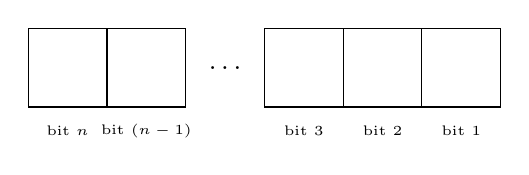
\begin{tikzpicture}
\draw (0,0) +(-.5,-.5) rectangle ++(.5,.5);
\draw (1,0) +(-.5,-.5) rectangle ++(.5,.5);
\draw (3,0) +(-.5,-.5) rectangle ++(.5,.5);
\draw (4,0) +(-.5,-.5) rectangle ++(.5,.5);
\draw (5,0) +(-.5,-.5) rectangle ++(.5,.5);
\draw (2,0) node{$\ldots$};
\draw (0,-.8) node{\tiny bit $n$};
\draw (1,-.8) node{\tiny bit $(n-1)$};
\draw (3,-.8) node{\tiny bit $3$};
\draw (4,-.8) node{\tiny bit $2$};
\draw (5,-.8) node{\tiny bit $1$};
\end{tikzpicture}
\end{center}
\begin{itemize}
\item Singolo bit ({\bf b}inary dig{\bf it})  assume solo valori $0$ o $1$
\item Memoria a $n$ bit? $2^n$ configurazioni
\item Rappresentare i naturali? Sistema posizionale\\
Con $n$ bit, rappresento range $\{ 0 , 1 , \ldots , 2^{n}-1 \} \subset \mathbb{N}$
\item Rappresentare gli interi? Idee?
\item Un bit per il segno, il resto posizionale?
\item Non compatto e no somma in colonna
\item Metodo alternativo: complemento a due!
\end{itemize}
\end{column}
\begin{column}[T]{0.3\textwidth}
\setbeamercovered{}
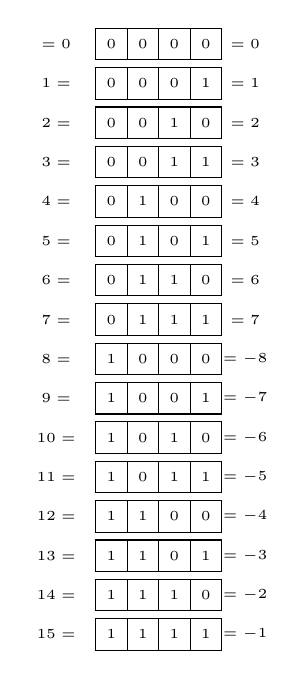
\begin{tikzpicture}
\draw (0,0) +(-.2,-.2) rectangle ++(.2,.2); \draw (0,0) node{\tiny $1$};
\draw (.4,0) +(-.2,-.2) rectangle ++(.2,.2); \draw (.4,0) node{\tiny $1$};
\draw (.8,0) +(-.2,-.2) rectangle ++(.2,.2); \draw (.8,0) node{\tiny $1$};
\draw (1.2,0) +(-.2,-.2) rectangle ++(.2,.2); \draw (1.2,0) node{\tiny $1$};
\draw (0,.5) +(-.2,-.2) rectangle ++(.2,.2); \draw (0,.5) node{\tiny $1$};
\draw (.4,.5) +(-.2,-.2) rectangle ++(.2,.2); \draw (.4,.5) node{\tiny $1$};
\draw (.8,.5) +(-.2,-.2) rectangle ++(.2,.2); \draw (.8,.5) node{\tiny $1$};
\draw (1.2,.5) +(-.2,-.2) rectangle ++(.2,.2); \draw (1.2,.5) node{\tiny $0$};
\draw (0,1) +(-.2,-.2) rectangle ++(.2,.2); \draw (0,1) node{\tiny $1$};
\draw (.4,1) +(-.2,-.2) rectangle ++(.2,.2); \draw (.4,1) node{\tiny $1$};
\draw (.8,1) +(-.2,-.2) rectangle ++(.2,.2); \draw (.8,1) node{\tiny $0$};
\draw (1.2,1) +(-.2,-.2) rectangle ++(.2,.2); \draw (1.2,1) node{\tiny $1$};
\draw (0,1.5) +(-.2,-.2) rectangle ++(.2,.2); \draw (0,1.5) node{\tiny $1$};
\draw (.4,1.5) +(-.2,-.2) rectangle ++(.2,.2); \draw (.4,1.5) node{\tiny $1$};
\draw (.8,1.5) +(-.2,-.2) rectangle ++(.2,.2); \draw (.8,1.5) node{\tiny $0$};
\draw (1.2,1.5) +(-.2,-.2) rectangle ++(.2,.2); \draw (1.2,1.5) node{\tiny $0$};
\draw (0,2) +(-.2,-.2) rectangle ++(.2,.2); \draw (0,2) node{\tiny $1$};
\draw (.4,2) +(-.2,-.2) rectangle ++(.2,.2); \draw (.4,2) node{\tiny $0$};
\draw (.8,2) +(-.2,-.2) rectangle ++(.2,.2); \draw (.8,2) node{\tiny $1$};
\draw (1.2,2) +(-.2,-.2) rectangle ++(.2,.2); \draw (1.2,2) node{\tiny $1$};
\draw (0,2.5) +(-.2,-.2) rectangle ++(.2,.2); \draw (0,2.5) node{\tiny $1$};
\draw (.4,2.5) +(-.2,-.2) rectangle ++(.2,.2); \draw (.4,2.5) node{\tiny $0$};
\draw (.8,2.5) +(-.2,-.2) rectangle ++(.2,.2); \draw (.8,2.5) node{\tiny $1$};
\draw (1.2,2.5) +(-.2,-.2) rectangle ++(.2,.2); \draw (1.2,2.5) node{\tiny $0$};
\draw (0,3) +(-.2,-.2) rectangle ++(.2,.2); \draw (0,3) node{\tiny $1$};
\draw (.4,3) +(-.2,-.2) rectangle ++(.2,.2); \draw (.4,3) node{\tiny $0$};
\draw (.8,3) +(-.2,-.2) rectangle ++(.2,.2); \draw (.8,3) node{\tiny $0$};
\draw (1.2,3) +(-.2,-.2) rectangle ++(.2,.2); \draw (1.2,3) node{\tiny $1$};
\draw (0,3.5) +(-.2,-.2) rectangle ++(.2,.2); \draw (0,3.5) node{\tiny $1$};
\draw (.4,3.5) +(-.2,-.2) rectangle ++(.2,.2); \draw (.4,3.5) node{\tiny $0$};
\draw (.8,3.5) +(-.2,-.2) rectangle ++(.2,.2); \draw (.8,3.5) node{\tiny $0$};
\draw (1.2,3.5) +(-.2,-.2) rectangle ++(.2,.2); \draw (1.2,3.5) node{\tiny $0$};
\draw (0,4) +(-.2,-.2) rectangle ++(.2,.2); \draw (0,4) node{\tiny $0$};
\draw (.4,4) +(-.2,-.2) rectangle ++(.2,.2); \draw (.4,4) node{\tiny $1$};
\draw (.8,4) +(-.2,-.2) rectangle ++(.2,.2); \draw (.8,4) node{\tiny $1$};
\draw (1.2,4) +(-.2,-.2) rectangle ++(.2,.2); \draw (1.2,4) node{\tiny $1$};
\draw (0,4.5) +(-.2,-.2) rectangle ++(.2,.2); \draw (0,4.5) node{\tiny $0$};
\draw (.4,4.5) +(-.2,-.2) rectangle ++(.2,.2); \draw (.4,4.5) node{\tiny $1$};
\draw (.8,4.5) +(-.2,-.2) rectangle ++(.2,.2); \draw (.8,4.5) node{\tiny $1$};
\draw (1.2,4.5) +(-.2,-.2) rectangle ++(.2,.2); \draw (1.2,4.5) node{\tiny $0$};
\draw (0,5) +(-.2,-.2) rectangle ++(.2,.2); \draw (0,5) node{\tiny $0$};
\draw (.4,5) +(-.2,-.2) rectangle ++(.2,.2); \draw (.4,5) node{\tiny $1$};
\draw (.8,5) +(-.2,-.2) rectangle ++(.2,.2); \draw (.8,5) node{\tiny $0$};
\draw (1.2,5) +(-.2,-.2) rectangle ++(.2,.2); \draw (1.2,5) node{\tiny $1$};
\draw (0,5.5) +(-.2,-.2) rectangle ++(.2,.2); \draw (0,5.5) node{\tiny $0$};
\draw (.4,5.5) +(-.2,-.2) rectangle ++(.2,.2); \draw (.4,5.5) node{\tiny $1$};
\draw (.8,5.5) +(-.2,-.2) rectangle ++(.2,.2); \draw (.8,5.5) node{\tiny $0$};
\draw (1.2,5.5) +(-.2,-.2) rectangle ++(.2,.2); \draw (1.2,5.5) node{\tiny $0$};
\draw (0,6) +(-.2,-.2) rectangle ++(.2,.2); \draw (0,6) node{\tiny $0$};
\draw (.4,6) +(-.2,-.2) rectangle ++(.2,.2); \draw (.4,6) node{\tiny $0$};
\draw (.8,6) +(-.2,-.2) rectangle ++(.2,.2); \draw (.8,6) node{\tiny $1$};
\draw (1.2,6) +(-.2,-.2) rectangle ++(.2,.2); \draw (1.2,6) node{\tiny $1$};
\draw (0,6.5) +(-.2,-.2) rectangle ++(.2,.2); \draw (0,6.5) node{\tiny $0$};
\draw (.4,6.5) +(-.2,-.2) rectangle ++(.2,.2); \draw (.4,6.5) node{\tiny $0$};
\draw (.8,6.5) +(-.2,-.2) rectangle ++(.2,.2); \draw (.8,6.5) node{\tiny $1$};
\draw (1.2,6.5) +(-.2,-.2) rectangle ++(.2,.2); \draw (1.2,6.5) node{\tiny $0$};
\draw (0,7) +(-.2,-.2) rectangle ++(.2,.2); \draw (0,7) node{\tiny $0$};
\draw (.4,7) +(-.2,-.2) rectangle ++(.2,.2); \draw (.4,7) node{\tiny $0$};
\draw (.8,7) +(-.2,-.2) rectangle ++(.2,.2); \draw (.8,7) node{\tiny $0$};
\draw (1.2,7) +(-.2,-.2) rectangle ++(.2,.2); \draw (1.2,7) node{\tiny $1$};
\draw (0,7.5) +(-.2,-.2) rectangle ++(.2,.2); \draw (0,7.5) node{\tiny $0$};
\draw (.4,7.5) +(-.2,-.2) rectangle ++(.2,.2); \draw (.4,7.5) node{\tiny $0$};
\draw (.8,7.5) +(-.2,-.2) rectangle ++(.2,.2); \draw (.8,7.5) node{\tiny $0$};
\draw (1.2,7.5) +(-.2,-.2) rectangle ++(.2,.2); \draw (1.2,7.5) node{\tiny $0$};

\draw (-.7,0) node{\tiny $15=$}; \draw (-.7,.5) node{\tiny $14=$}; \draw (-.7,1) node{\tiny $13=$}; \draw (-.7,1.5) node{\tiny $12=$}; \draw (-.7,2) node{\tiny $11=$}; \draw (-.7,2.5) node{\tiny $10=$}; \draw (-.7,3) node{\tiny $9=$}; \draw (-.7,3.5) node{\tiny $8=$}; \draw (-.7,4) node{\tiny $7=$}; \draw (-.7,4.5) node{\tiny $6=$}; \draw (-.7,5) node{\tiny $5=$}; \draw (-.7,5.5) node{\tiny $4=$}; \draw (-.7,6) node{\tiny $3=$}; \draw (-.7,6.5) node{\tiny $2=$}; \draw (-.7,7) node{\tiny $1=$}; \draw (-.7,7.5) node{\tiny $= 0$};
\draw (1.7,0) node{\tiny $= -1$}; \draw (1.7,.5) node{\tiny $= -2$}; \draw (1.7,1) node{\tiny $= -3$}; \draw (1.7,1.5) node{\tiny $= -4$}; \draw (1.7,2) node{\tiny $= -5$};
\draw (1.7,2.5) node{\tiny $= -6$}; \draw (1.7,3) node{\tiny $= -7$}; \draw (1.7,3.5) node{\tiny $= -8$}; \draw (1.7,4) node{\tiny $= 7$}; \draw (1.7,4.5) node{\tiny $= 6$};
\draw (1.7,5) node{\tiny $= 5$}; \draw (1.7,5.5) node{\tiny $= 4$}; \draw (1.7,6) node{\tiny $= 3$}; \draw (1.7,6.5) node{\tiny $= 2$}; \draw (1.7,7) node{\tiny $= 1$}; \draw (1.7,7.5) node{\tiny $= 0$};

\end{tikzpicture}
\end{column}
\end{columns}}



\end{document}
